\documentclass{../../vmdm}

\begin{document}
\boxedpoints

\VMDMTitre{novembre 2022 (6ème)}
\vspace{0.2cm}
\VMDMRegles{}
\vspace{0.2cm}

\qformat{Exercice \thequestion \dotfill (\totalpoints~points)}
\begin{questions}
    \question[4]
    \begin{parts}
        \part
        \begin{subparts}
            \subpart Calculer $1 + 8 \times 1$ \hfill \rep{9}
            \subpart Calculer $2 + 8 \times 12$ \hfill\rep{98}
            \subpart Calculer $3 + 8 \times 123$ \hfill\rep{987}
        \end{subparts}
        \part Quel calcul permet d'obtenir \num{987654321} ? Vérifier.
    \end{parts}
    \question[10]
    Dans un triangle, la bissectrice d'un angle est une demi-droite qui coupe l'angle en deux angles égaux. Le schéma ci-dessous montre la bissectrice de l'angle $\widehat{BAC}$ en pointillé :
    \begin{center}
        \begin{tikzpicture}
            \coordinate (A) at (0,0);
            \coordinate (B) at (4,0);
            \coordinate (C) at ({2*cos(80)},{2*sin(80)});
            \draw (A) -- (B) -- (C) -- cycle;
            \draw[dashed] (A) -- ($(A)!3!({cos(40)}, {sin(40)})$);
            \node[below] at (A) {$A$};
            \node[below] at (B) {$B$};
            \node[left] at (C) {$C$};
            \draw[fill=black] (A) -- ($(A)!0.8!({cos(40)}, {sin(40)})$) arc (40:80:0.8) -- cycle;
            \draw[red,fill=red] (A) -- ($(A)!0.8!({cos(40)}, {sin(40)})$) arc (40:0:0.8) -- cycle;
            \node at (0.7,1) {\ang{40}};
            \node[red] at (1.2,0.4) {\ang{40}};
        \end{tikzpicture}
    \end{center}
    Sur ce schéma, l'angle $\widehat{BAC}$ qui mesure \ang{80} est coupé en deux angles de \ang{40} chacun par la bissectrice issue du point $A$.
    \begin{parts}
        \part Tracer un triangle $DEF$ tel que $DE = \qty{4}{\centi\metre}$, $EF = \qty{6}{\centi\metre}$ et $DF = \qty{8}{\centi\metre}$.
        \part Tracer les trois bissectrices du triangle (une partant du point $D$, une  autre partant du point $E$ et une dernière partant du point $F$). \\
        \textit{Si bien tracées, les trois bissectrices doivent concourir en un point $O$.}
        \part Tracer le \textit{cercle inscrit} du triangle $DEF$. Il s'agit du plus grand cercle qui satisfait les conditions suivantes :
        \begin{subparts}
            \subpart le cercle est à l'intérieur du triangle (il ne dépasse pas)
            \subpart le centre du cercle est le point $O$ (le point de concours des bissectrices)
        \end{subparts}
        \textit{Une fois tracé, on observera que le cercle << frôle >> les trois côtés du triangle. En mathématiques, on dit que le cercle est \emph{tangent} aux côtés du triangle.}
    \end{parts}
    \question[6]
    Un dé à 6 faces est un cube dont les 6 faces sont numérotées de 1 à 6. Toutefois, les numéros ne sont pas placés au hasard : lorsque l'on additionne les numéros de deux faces opposées, on obtient 7.
    \begin{center}
        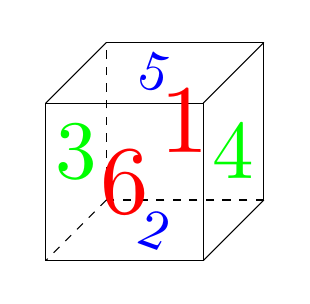
\begin{tikzpicture}
        	\draw[dashed] (2,0,0) -- (0,0,0) -- (0,2,0);
            \draw (0,2,0) -- (2,2,0) -- (2,0,0);
        	\draw (0,0,2) -- (0,2,2) -- (2,2,2) -- (2,0,2) -- cycle;
        	\draw[dashed] (0,0,0) -- (0,0,2);
        	\draw (0,2,0) -- (0,2,2);
        	\draw (2,0,0) -- (2,0,2);
        	\draw (2,2,0) -- (2,2,2);
            \node[scale=3.5,red] at (1,1,0) {1};
            \node[scale=2,blue,rotate=-20] at (1,0,1) {2};
            \node[scale=3,green] at (0,1,1) {3};
            \node[scale=3,green] at (2,1,1) {4};
            \node[scale=2,blue,rotate=-20] at (1,2,1) {5};
            \node[scale=3.5,red] at (1,1,2) {6};
        \end{tikzpicture}
    \end{center}
    Construire le patron de ce dé.
\end{questions}

\end{document}